\section{Validação}



\begin{enumerate}
\item Teste 1
\item Teste 2
\item Teste 3
\item Teste 4
\item Teste 5
\item Teste 6
\end{enumerate}

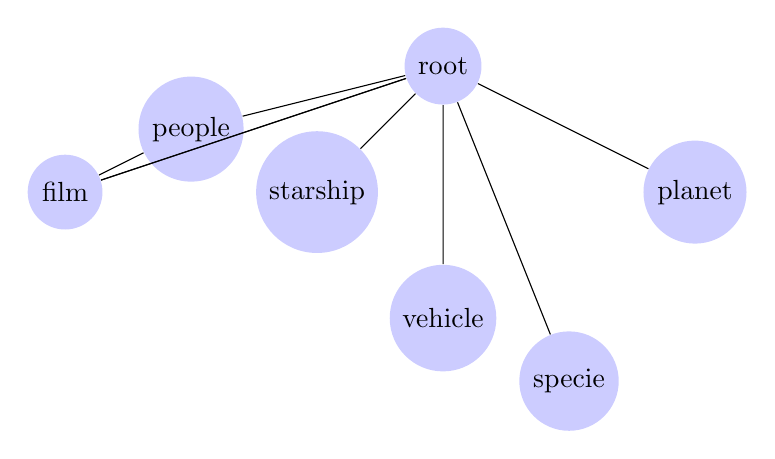
\begin{tikzpicture}
  [scale=.8,auto=left,every node/.style={circle,fill=blue!20}]
  \node (n1) at (6,10) {root};
  \node (n2) at (0,8)  {film};
  \node (n3) at (2,9)  {people};
  \node (n4) at (4,8) {starship};
  \node (n5) at (6,6)  {vehicle};
  \node (n6) at (8,5)  {specie};
  \node (n7) at (10,8)  {planet};

  \foreach \from/\to in {n1/n2,n1/n2,n1/n3,n1/n4,n1/n5,n1/n6,n1/n7,n2/n3}
    \draw (\from) -- (\to);

\end{tikzpicture}
